\begin{figure}[!tp]
    \centering
    \setlength{\abovecaptionskip}{4pt}
    \setlength{\belowcaptionskip}{0pt}
    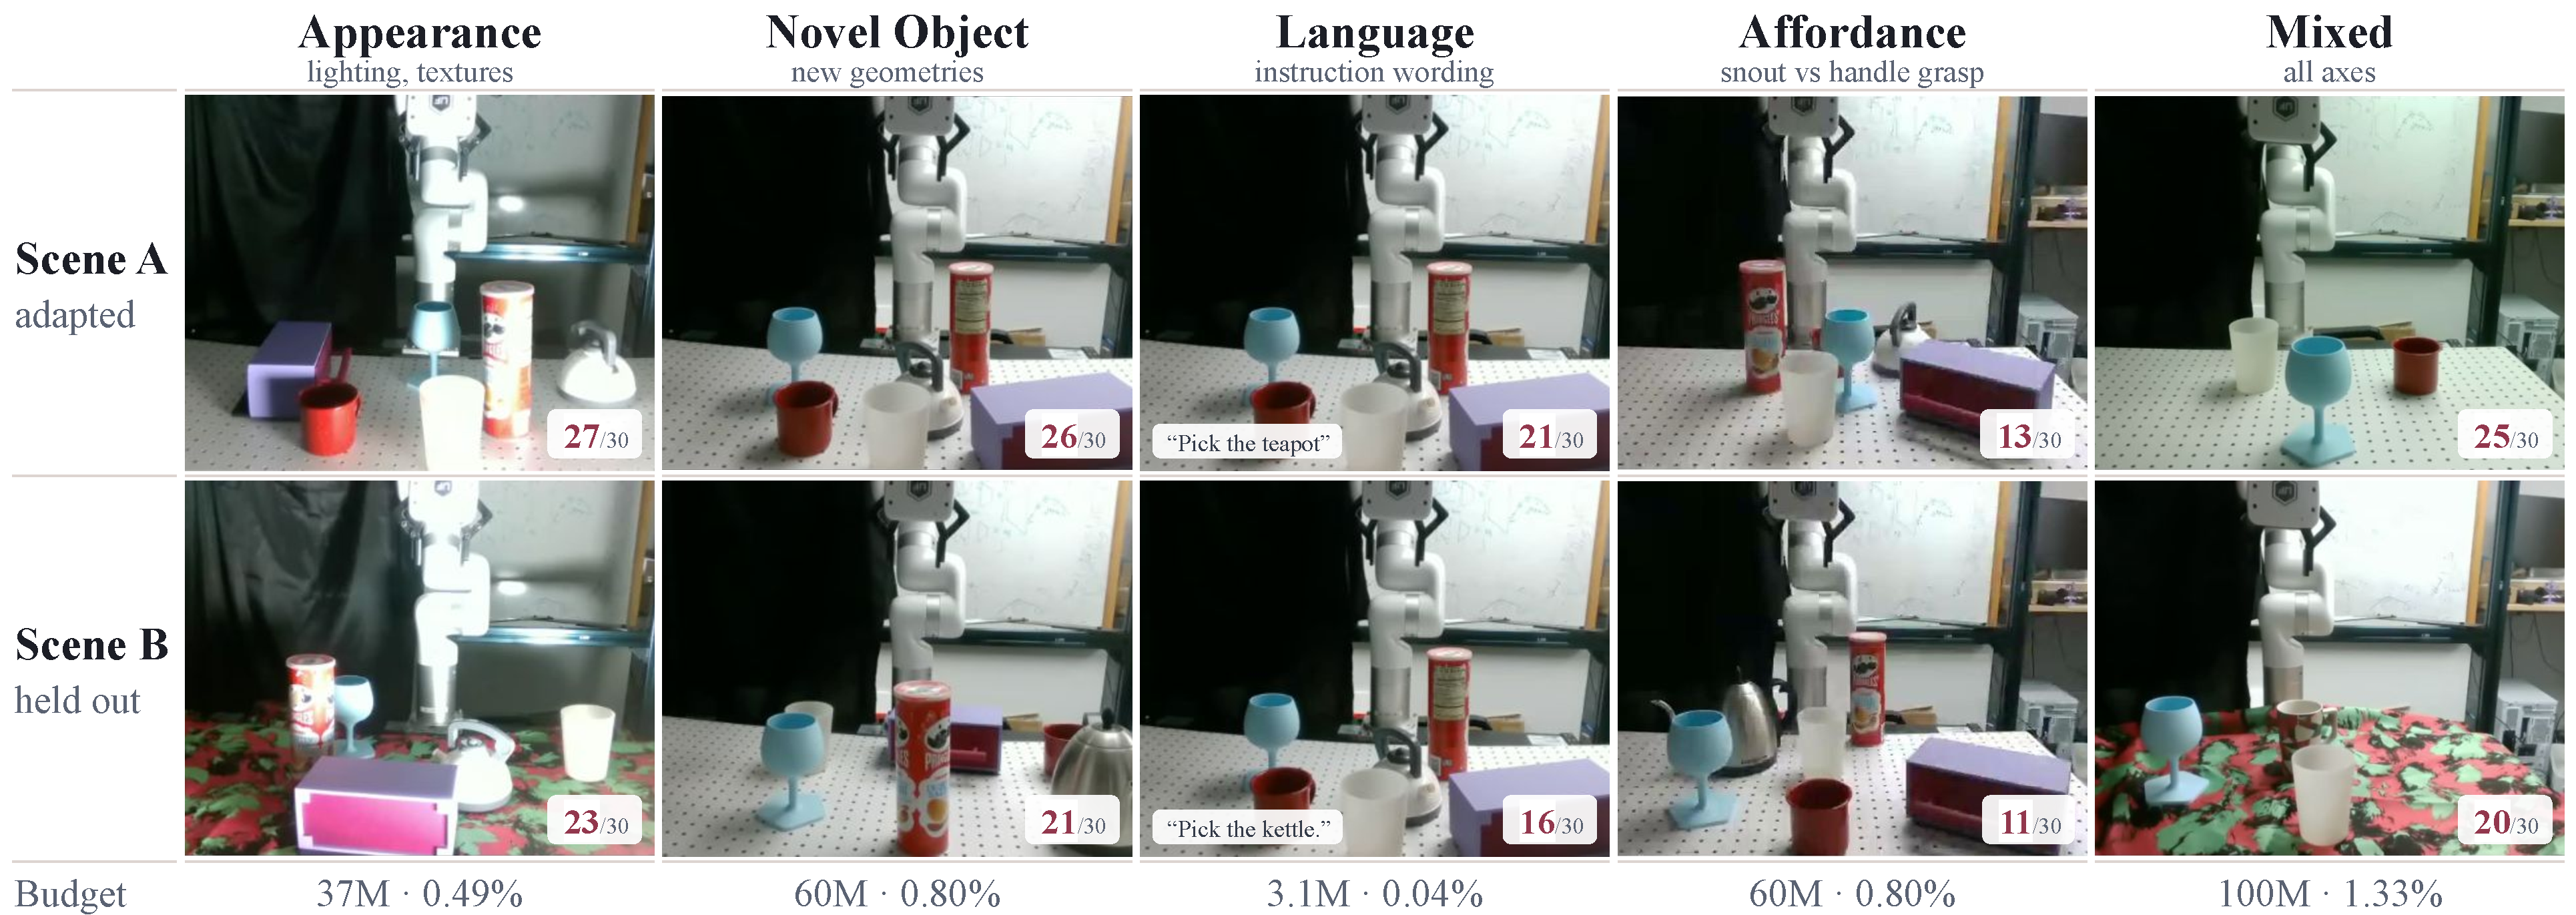
\includegraphics[width=\columnwidth]{images/physical_robot_figure.pdf}
    \caption{Five of the six xArm-7 shifts from the fixed third-person camera, with the adaptation condition (Scene~A, top) and the held-out condition (Scene~B, bottom) evaluated without retraining: appearance (lighting, then lighting plus background), novel object (toy and metallic teapot substitutions for the kettle), language (reworded instructions, with Scene~B naming the teapot), affordance (grasping the teapot by its snout rather than its handle), and mixed (a new cup geometry and color against a camouflaging background). Counts are Adaptive's successes of $30$ paired rollouts; the bottom row gives each shift's selected budget as a parameter count and a fraction of the $7.5$B policy.}
    \label{fig:physical-scenes}
\end{figure}